\section{Literature review}
\label{sec:lit_review}

In this section, I review the existing literature on how governments influence the media and manipulate the information environment to achieve electoral advantages. This discussion covers strategies observed in both authoritarian and democratic contexts, as well as those specific to the Mexican political landscape.

\subsection{Authoritarian Regimes}

In authoritarian contexts, governments exercise control over the media in two main ways. The first is by allocating substantial resources to control the information environment through censorship. For example, in China, \cite{Army-Chen-Book} and \citep{CensorshipCollective-King-APSR} document that each internet content provider employs thousands of censors to ensure compliance with government regulations, while the government itself deploys an extensive force of over 300,000 cyber-police to oversee censorship efforts. As described by \cite{CensorshipChina-King-Science}, this represents the largest recorded suppression of free expression in history. Notably, their seminal work shows that this censorship primarily targets posts indicative of collective action, while government criticism is generally allowed.

The second method of control is through personnel management. For instance, \cite{Plus-Anne-PostComm} note that the Chinese government directly controls the appointment of managers and editors within the media, while \cite{PersonnelMedia-Lee-IntJPPoli} highlight that dictators selectively promote aligned journalists to shape the content of news reports. Finally, some theoretical and empirical evidence suggest that in resource-scarce dictatorships, governments may be more inclined to permit greater press freedom as a means of gathering information about their bureaucrats \citep{PoorDict-Guriev-APSR} and power-sharing elites \citep{ElitesMedia-Tung-PolComm}. This approach allows the government to monitor and control these groups, helping to prevent crises and maintain stability.

\subsection{Democracies}

In well-functioning democracies, evidence of such practices is more limited. However, while these tactics are more nuanced, governments and elites still employ them to gain control over the information environment and influence media reporting.\footnote{By \textit{well-functioning democracies}, I refer to countries with a comprehensive set of democratic mechanisms, such as a constitution, regular elections, a free press, and opposition parties, among others. Given that the level of democratization varies widely across countries, I provide examples and differentiate between developing nations and industrialized democracies.} In this context, one common strategy employed by leaders is to delegitimize the media. There is substantial evidence that this tactic affects how individuals perceive media bias and damages the media’s overall reputation \citep{PercMedia-Egelholfer-JoComm, PolNews-Smith-JoPressPol}, which could in consequence affect their reporting. Moreover, this approach is not limited to developing countries \citep{JournIndia-Bhat-Dig, ThugMex-VictorHugo-JourPract}; it is also widespread in industrialized democracies \citep{KoreaJour-Shin-Journalism, PressCriticism-Carlson-Journalism}. In recent years, with the rise of populism, the use of this strategy has become more pronounced, further shaping public perception of the media \citep{PolEconPop-Guriev-JEL}.

Another tactic employed by governments to control the media is bribery. \cite{Peru-Macmillan-JEP} document how Montesinos, the intelligence officer under Fujimori, paid millions of dollars in bribes to media owners, opposition politicians, and judges. In some cases, these bribes were used to gain full control over media broadcasts for specific periods. Notably, and in support of my argument about the significance of the information environment, the amounts paid to media owners were exponentially higher—100 times greater—than those paid to judges and politicians.

Politicians and governments can also shape media reporting through legal mechanisms that require minimal resources. These include laws that restrict free speech \citep{MexicanPressStanigAJPS, Journalism-Salazar-RevMex}, limit access to sources \citep{Kisha-UoNott, Kisha-Freedom}, or regulate media licensing \citep{PolicyBrief-MediaRegulation}. Related with laws that restrict free speech in Mexico, \cite{MexicanPressStanigAJPS} analyzes cross-state variations in the strictness of speech regulations to show that media outlets report less on government corruption in regions where speech is more tightly controlled. This trend is largely driven by journalists' fear of prosecution or defamation lawsuits. Using a similar approach, \cite{Journalism-Salazar-RevMex} finds that this effect is mediated by the level of judiciary independence in each state.

Finally and in close relation with this line of research, \cite{ArgCorr-DiTella-AEJAE} find—for the case of Argentina's newspapers—that advertising spending and media coverage of corruption scandals is negatively correlated, meaning that increases in advertising spending are associated with a decrease in critical coverage of the government. 

\subsection{The Mexican Context}

Historical, observational, and anecdotal evidence has extensively documented the tactics used by the Mexican government to control the information environment and suppress dissent through its relationship with the media. Since the early 1900s, the media-government relationship has been characterized by collusion, particularly during the PRI’s rule, where both, the elites and the government, worked to preserve the status quo. As \cite{FourthState-Lawson-Book} highlights, media owners benefited from economic incentives like tax exemptions and broadcasting concessions, while mid-level managers and journalists received \textit{chayote} (a common form of bribery). This allowed the government to manage narratives without resorting to overt repression. Advertising spending was also strategically used to secure favorable coverage, as demonstrated by President López Portillo's withdrawal of funding from independent media outlets, famously stating, \textit{"Pay for them to beat up on me? Gentlemen, I think not!"} \citep{PrensaVendida-Rod}.

The democratic transition of the 1990s brought changes, with independent media and the Federal Electoral Institute (\textit{IFE}) contributing to significant political shifts, such as Cuauhtémoc Cárdenas’s win in Mexico City in 1997 and Andrés Manuel López Obrador's (AMLO) victory in 2000. However, old tactics persisted. Under Calderón, given the increase in violence due to the War on Drugrs, media cooperation was framed as necessary to avoid aiding criminal organizations. In 2011, a meeting convened by Televisa and TV Azteca led to 715 media outlets agreeing to editorial guidelines that would “\textit{not benefit criminal organizations}” \citep{Callaron-Jornada, Callaron-Proceso}. Meanwhile, advertising spending soared, with a 501\% increase in 2009 compared to the last year of Vicente Fox's presidency \citep{Fundar}, often funded through illegal resource diversions, such as 1.5 billion pesos channeled from the Ministry of Health \citep{Contralinea-Desvio}.

During Enrique Peña Nieto's presidency, these strategies intensified. Advertising spending was wielded as a tool to control media narratives, with outlets refraining from criticism to secure government funding. For instance, in 2017, The New York Times published an article titled "\textit{Using Billions in Government Cash, Mexico Controls News Media}" where they documented all this tactics through interviews with editors, reporters and managers \citep{Times}. High-profile cases, like the removal of a \textit{Milenio} story critical of anti-poverty program mismanagement \citep{Milenio-Buzz}, highlighted this control. The firing of journalist Carmen Aristegui after exposing the \textit{White House} corruption scandal and the murder of a \textit{Proceso} photographer further emphasized the PRI's reliance on both financial control and intimidation to suppress dissent \citep{WashPost-Aristegui, Times2-Kill}.


In 2018, Andrés Manuel López Obrador, the candidate for the newly formed MORENA party, won the presidential election, marking a significant shift in the relationship between the government and the media. Under his administration’s policy of republican austerity, government spending on advertising was drastically reduced by 78.7\%, a move that likely influenced media coverage and their stance on various issues \citep{Article19, ElEconomist-Republican}. Figure \ref{fig:yearly_spending} illustrates this sharp decrease in advertising expenditure.

\begin{figure}[!htpb]
   \centering
   \small
   \caption{Evolution of the approved and exerted spending in government advertising spending}
   \label{fig:yearly_spending}
   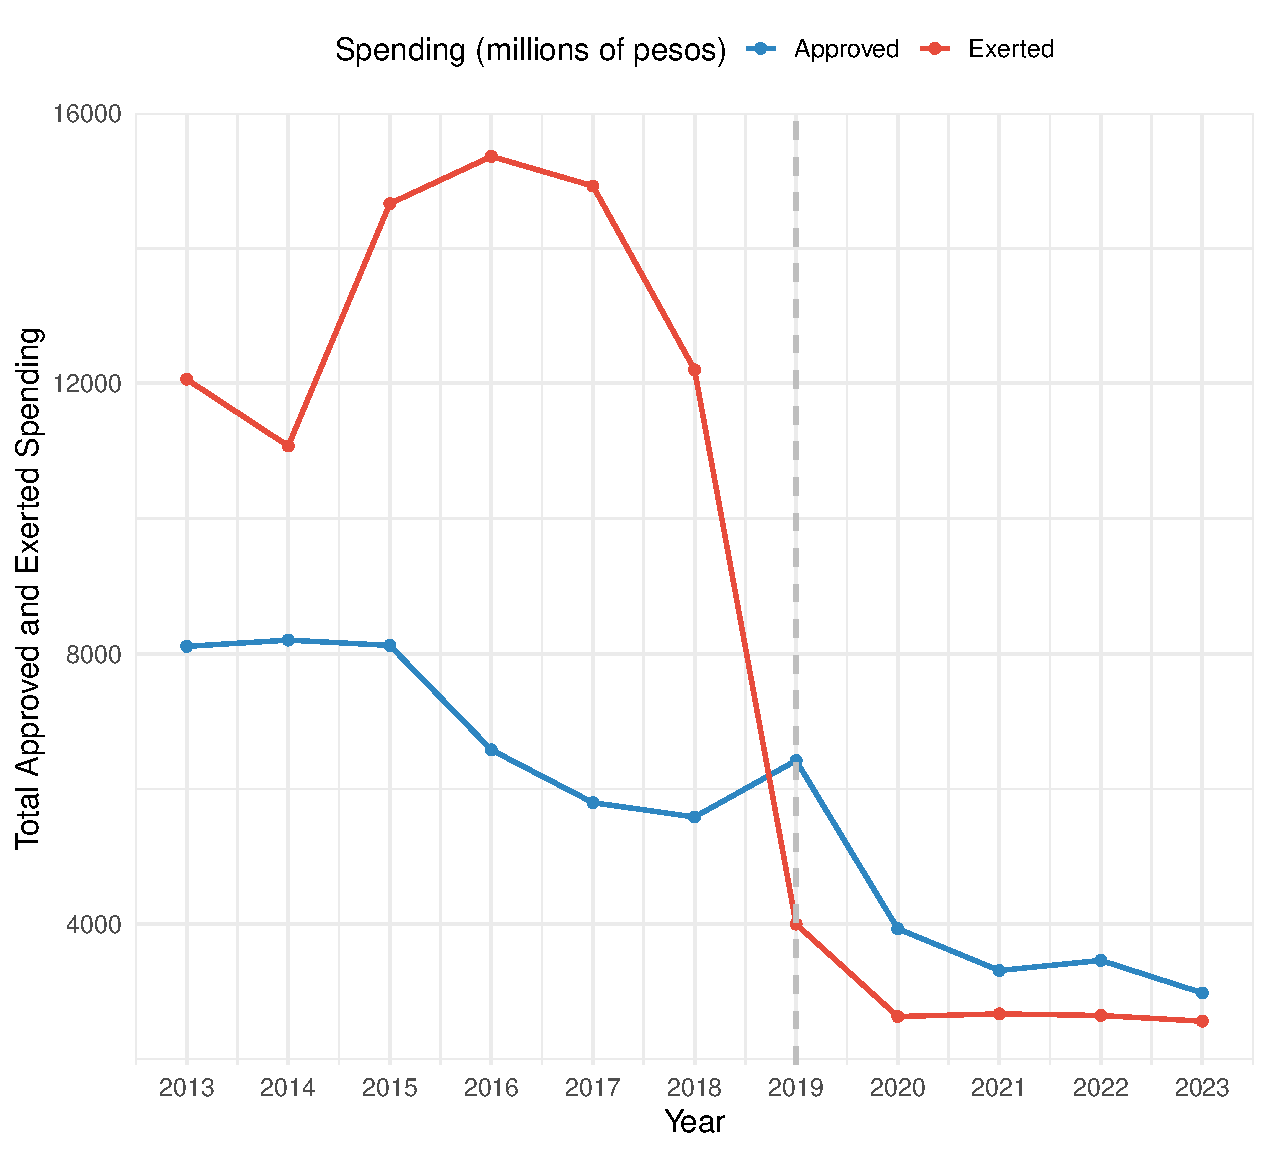
\includegraphics[width=.9\textwidth]{figures/descriptive_stats/ppto_article19.pdf}
   \caption*{ \footnotesize{\textit{Note:} This figure presents the yearly line trend (2012-2023) for the social advertising spending (on millions of pesos) from the Mexican government, divided by the spending approved by the Chamber of Deputies and the Senate at the beginning of that year (Blue) and the actual exerted spending (Red). The grey line represents the start of AMLO's tenure. Data was obtained from COMSOC and \citep{Article19}.}}
\end{figure}

This decrease in government spending, however, did not result in a more transparent or equitable system for allocating these resources. \cite{Article19} highlights that although the budget for this area was reduced, the absence of a robust regulatory framework has allowed the distribution of funds to remain highly discretionary. Journalistic investigations have also revealed that the decrease in spending was accompanied by a discretionary reallocation of resources, shifting funds away from right-wing opposition outlets to those more aligned with the administration’s left-wing agenda.

Two notable examples illustrate this trend. The first is Nexos, a right-wing opinion magazine that lost its entire advertising budget when AMLO took office.\footnote{This conclusion is based on an analysis of COMSOC data.} The second is the significant increase in advertising directed toward aligned southern outlets, such as \textit{Grupo Cantón} and \textit{Compañía Editorial del Mayab}, whose CEO's mentioned in several occasions that they held a good relationship with AMLO \citep{Animal-Discrecionalidad}.

In addition, López Obrador introduced daily morning press conferences, where he engaged directly with the media every weekday. These sessions were used to address pressing issues, express his thoughts, criticize opposition parties and figures, and respond to questions from the press and public. This unprecedented level of accessibility reshaped the interaction between the government and the media, creating a new dynamic in political communication \citep{ThugMex-VictorHugo-JourPract}.

While these press conferences had the potential to serve as an accountability tool, many scholars and journalists contend that they primarily functioned as a vehicle for government propaganda. Critics argue that the President used these platforms to disseminate misleading narratives, reinforce support for his administration, and publicly attack opponents and dissenting voices \citep{OtrosDatos}. 

In conclusion, the historical and anecdotal evidence strongly suggests that advertising spending has been the government’s primary tool for securing favorable media coverage, silencing critics, and ultimately exerting greater control over the information environment. Given this context---and the potential to identify exogenous variation in the number of critical articles written by media outlets---it becomes interesting to ask whether this administration continues to use advertising spending for these purposes, as well as to analyze the magnitude of its impact and the mechanisms underlying this practice.